\documentclass[10pt, a4paper]{article}
\usepackage{authblk}
\usepackage{lrec2014}
\usepackage{url}
\usepackage{latexsym}

\usepackage{fontspec}
\usepackage{xunicode}
\usepackage{xltxtra}


\setmainfont[Mapping=tex-text]{Times New Roman}

\title{Heuristic Hyper-minimization of Finite State Lexicons}

% ----------------------------------------------------------------------
% AUTHOR FORMATS
% 
% ------------
% For several authors from the same institution:
%
% \name{Firstname1 Surname1, Firstname2 Surname2, ..., FirstnameN SurnameN}
%
% \address{Institution \\ Address \\ {mail1, mail2, ...,  mailN}@institution}
%
% If the names do not fit well on one line use
%
%         \name{Firstname1 Surname1 \\ {\bf \large Firstname2 Surname2} \\
%         ... \\ {\bf \large FirstnameN SurnameN }}
%
% ------------
%
% For authors from different institutions:
%
% \name{Firstname1 Surname1$^{\ast}$, Firstname2 Surname2$^{\ast}$, Firstname3 Surname3$^{\dagger}$, Firstname4 Surname4$^{\ast}$}
%
% \address{$^{\ast}$Institution1 \\ Address1 \\ 
%          {mail1, mail2, mail4}@Institution1} \\ \\
%          $^{\dagger}$Institution2 \\ Address3 \\ 
%          mail3@Institution2 }
%
% ------------



\name{Senka Drobac$^{\ast}$, Krister Lind\'{e}n$^{\ast}$, Tommi A Pirinen$^{\dagger}$, Miikka Silfverberg$^{\ast}$}
\address{$^{\ast}$University of Helsinki \\ Department of Modern Languages, PO Box 24 \\ 
$^{\dagger}$University of Helsinki \\ Department of Speech Sciences, PO Box 9 \\
{senka.drobac, kriste.linden, tommi.pirinen, miikka.silfverberg}@helsinki.fi\\}





\iffalse
\author[1]{Senka Drobac}
\author[1]{Krister Lind\'{e}n}
\author[2]{Tommi A Pirinen}
\author[1]{Miikka Silfverberg}
\affil[1]{Department of Modern Languages, PO Box 24, 00014 University of Helsinki}
\affil[2]{Department of Speech Sciences, PO Box 9, 00014 University of Helsinki}

\renewcommand\Authands{ and }
\fi

\abstract{Flag diacritics enable optimising finite-state networks by
    combining identical sub-graphs of its transition
    graph. Traditionally, the feature has required linguists to devise
    the optimisations to the graph by hand alongside the morphological
    description. In this paper, we present a novel method of
    discovering flag positions in morphological lexicons automatically
    based on the morpheme structure implicit in the language
    description. With this approach, we have gained significant
    decrease in the size of finite-state networks while maintaining reasonable application 
    speed. ... (150-200 words) \\ \newline \Keywords{hyper-minimization, lexicons, keyword C}}

%TODO - write more in abstract, keywords!

\date{\today}

\begin{document}
\maketitleabstract


\section{Introduction}

Finite-state transducers are an established way of encoding
morphological analysers for natural languages. Nevertheless,
full-scale morphological analysers can often grow to be too large for
use cases like spell checkers, speech processing and shallow parsing, which 
should have moderate memory footprint. Large transducers can be optimised by preserving the sub-lexicon structure with special symbols called flag diacritics, which prevents combinatorial blow ups in determinization.

%Large transducers can be optimised by recognising equivalent sub-graphs and combining them by using special symbols called flag diacritics, to couple entrance points of the sub-graphs with the correct exit points.

Up to date, applying flag diacritics has required a linguist to provide
the lexicon compiler with their positions. However, there are two
major problems with this kind of approach: Firstly, linguists often do
not have a very good understanding of the structure of the
finite-state networks built from lexicographical-morphological
descriptions; Secondly, the addition of flag diacritics to these
descriptions makes them unreadable and unmanageable since the amount
of non-linguistic data in the linguistic description increases. 

One of the reasons why flag diacritics have been so cumbersome from
the linguists point of view, is their two-fold nature. On one hand,
they are there to optimise the finite-state automaton structure,
e.g. in~\cite{karttunen2006numbers}. On the other hand, they are the
primary method of describing non-contiguous morphological
constraints~\cite{beesley1998constraining}. If they are applied on the
constriction of separated morphotactic dependencies, the effect on
optimisation is at best haphazard, and the resulting description is
neither linguistically motivated nor maintainable from a computational
view-point.

This article seeks to address problems associated with flag diacritics
by using an algorithm for inducing flag positions from the linguistic
morpheme structure, implicitly present in lexical
descriptions.

\begin{figure*}
    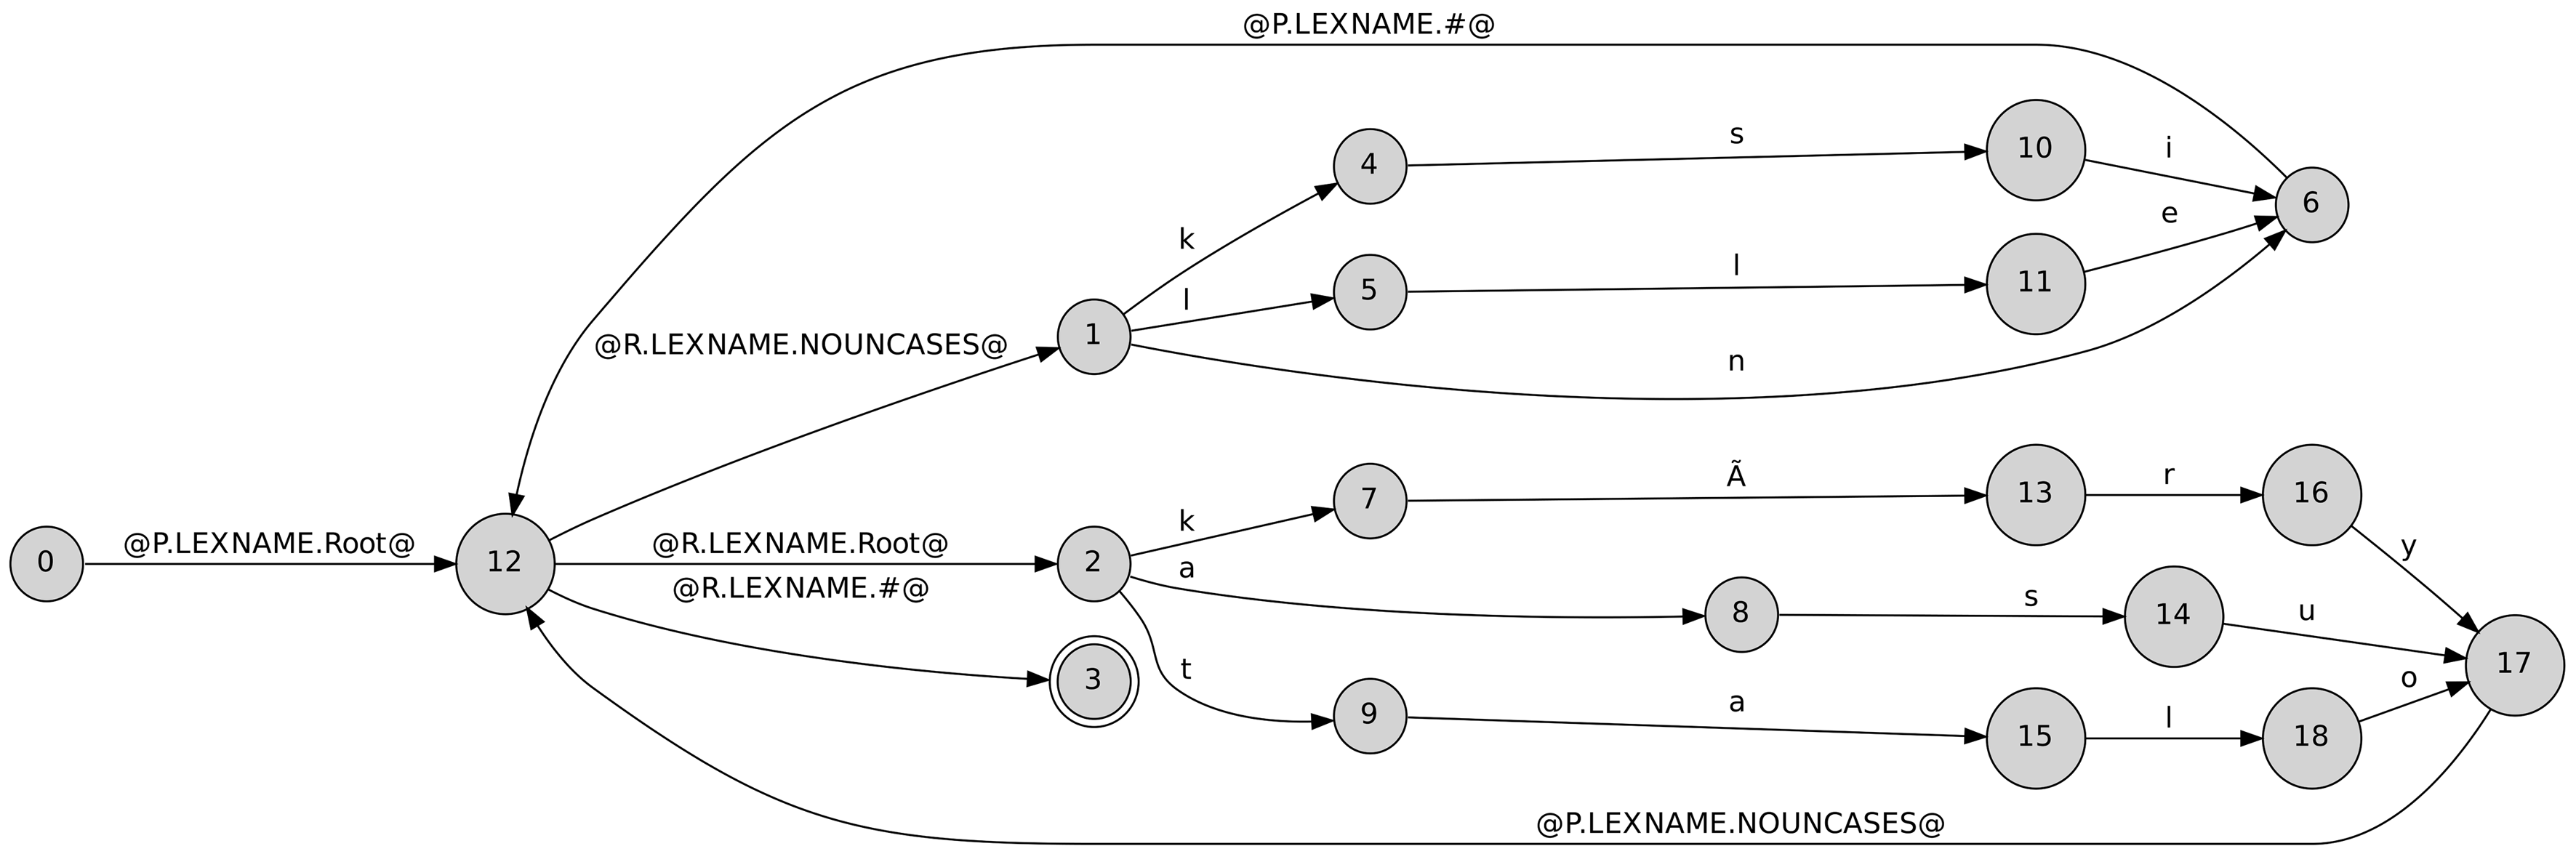
\includegraphics[width=\textwidth]{transducer.png}
     \caption{Simplified part of Finnish lexc grammar description with automatic flags
     \label{fig:lexc-fin-flag}}
\end{figure*}

\begin{figure*}
    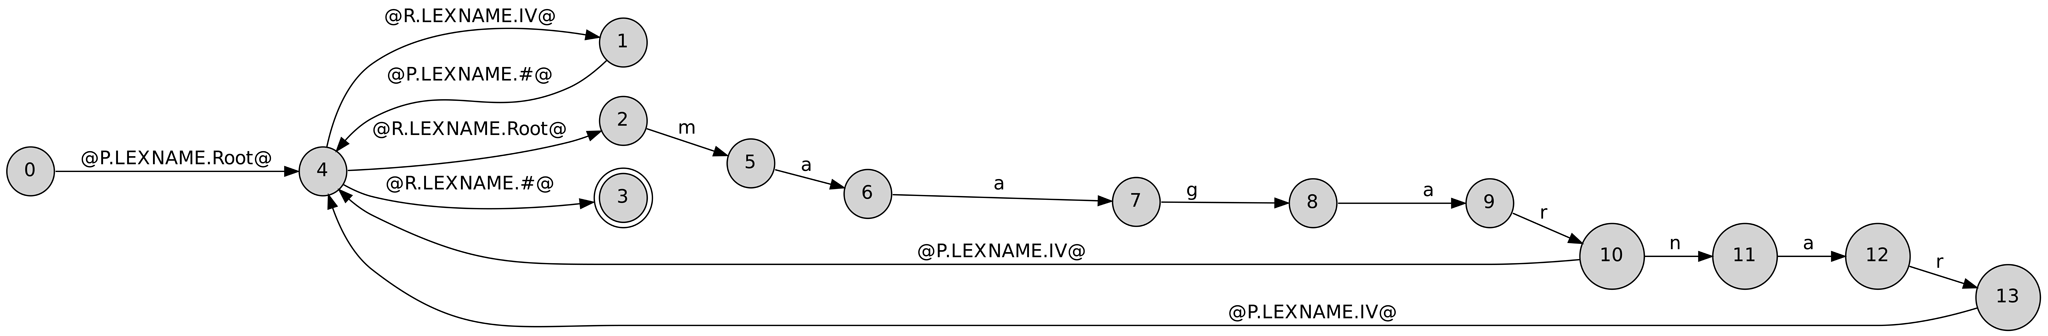
\includegraphics[width=\textwidth]{gr.png}
     \caption{Simplified part of Greenlandic lexc grammar description with automatic flags
     \label{fig:lexc-gr-flag}}
\end{figure*}

\section{Background}

\label{sec:background}

Finite state morphology~\cite{beesley2003finite} is the
state-of-the-art in writing morphological analysers for natural
languages of the whole range of typologically varying morphological
features. The finite-state approach is built around two practical
concepts: constructing lexicographical descriptions of the language
using a syntax called lexc and expressing morphophonological
variations as regular expression rules. In this paper we study the use
of lexicographical structure as framed by lexc. 

Lexc is a simple right-linear phrase structure grammar formalism. In
linguistic terms this means approximately the following: we have
collections of lexicons, which are lists of morphemes. Each morpheme
in a lexicon defines a continuation lexicon, which in turn determines
the set of morphemes that can succeed the original morpheme and their
possible continuations.

Consider for example Finnish morphology. Nominal inflection can be
constructed neatly from left to right. In figure~\ref{fig:lexc-fin},
there is a lexc representation of the Finnish words \emph{talo} `house',
\emph{asu} `clothing' and \emph{kärry} `cart', and nominal suffixes
\emph{n} (singular genitive), \emph{lle} (singular allative) and
\emph{ksi} (singular translative). Derivation of word-forms starts
from the \texttt{Root} lexicon. Each of the nouns in root set of morphemes
continues rightwards to \texttt{NOUNCASES} set of morphemes, and each
case morpheme continues towards the special \texttt{\#} lexicon
signifying the end of a word-form.




\begin{figure}
    \centering
    \begin{verbatim}
    LEXICON Root
    talo NOUNCASES ;
    asu NOUNCASES ;
    kärry NOUNCASES ;

    LEXICON NOUNCASES
    n # ;
    lle # ;
    ksi # ;
    \end{verbatim}
    \caption{Simplified part of Finnish lexc grammar description
    \label{fig:lexc-fin}}
\end{figure}

Finnish was used as an example in Karttunen's paper on flag diacritics
in optimisation~\shortcite{karttunen2006numbers}. In that paper, he
showed that the optimisation quality of wisely selected flag
diacritics can be substantial; from a 20,498 state automaton to an
1,946 state one. The article describes Finnish numerals, which have
the feature of requiring agreeing inflection in free compounding. This
can be achieved by allowing all compounds and restricting the
combinations by flags, instead by lexicon structure. Unfortunately,
the article does not show examples or re-producible description of the
lexicographical data, but to our experience there are no available
morphologies that show similar compression quality, so it can be
considered towards the upper bounds of what such compression can
achieve.
 
\section{Flag diacritics}
\label{sec:flags}

Flag diacritics are special multi-character symbols which are interpreted during runtime. They can be used to optimize large transducers to couple entrance points of the sub-graphs with the correct exit points.

Their special syntax is: \verb+@operator.feature.value@+, where
\texttt{operator} is one of the available operators (P, U, R, D, N, C), \texttt{feature} is name of a feature provisionally set by user and \texttt{value} can be any value held in feature, also provisionally defined ~\cite{beesley2003finite}.


In this paper, we will use only two types of flag diacritics: positive
setting (\verb+@P.feature.value@+) and require test
(\verb+@R.feature.value@+). While positive setting flag only sets the
feature to its value, require test flag invokes testing whether the
feature is set to the designated value.  For example,
\verb+@P.LEXNAME.Root@+ will set feature \texttt{LEXNAME} to value
\texttt{Root}. If later in the path there is an R flag that requires test
\verb+@R.LEXNAME.Root@+, the invoked test will succeed and that path
will be considered valid.



\section{Methods}
\label{sec:methods}

Our algorithm is based on the idea that adjacent morph combinatorics can be expressed with finite-state flags like this:

Every rightward continuation is replaced with a positive setting flag
with feature called \texttt{LEXNAME} and value corresponding to the
continuation lexicon. For example, the lexicon in
figure~\ref{fig:lexc-fin} has two rightward continuations:
\texttt{NOUNCASES} and \texttt{\#}, which are represented using flags
\verb+@P.LEXNAME.NOUNCASES@+ and \verb+@P.LEXNAME.#@+.  Similarly,
every leftward continuation is replaced with request test flag which
also has feature \texttt{LEXNAME} and the corresponding
value. Therefore, the lexicon shown in figure~\ref{fig:lexc-fin} will
also have two leftward continuations: \texttt{NOUNCASES} and
\texttt{\#}, which are represented using flags
\verb+@R.LEXNAME.NOUNCASES@+ and \verb+@R.LEXNAME.#@+. Additionally,
every morphological description starts with \texttt{Root}, which is
represented using the pair of flags
\verb+@P.LEXNAME.Root@@R.LEXNAME.Root@+.

The transducer built from the morphological description in
figure~\ref{fig:lexc-fin} is shown in figure~\ref{fig:lexc-fin-flag}.

\subsection{Composition}

Lexicons that contain flag diacritics can be composed with other
transducers which also contain flag diacritics without worrying about
flag collisions. This is achieved by renaming flag diacritics in both
argument transducers in such a way that collisions become impossible
and then inserting flag diacritics freely from each argument to the
other.

Consider for example composition of a lexicon $L$ with a rule $R$. If
both transducers contain flag diacritics for feature {\tt FEATURE},
then $all features F$ are renamed {\tt F1} in $L$ and {\tt F2} in
$R$.~\footnote{It is not sufficient to rename only flag diacritics
  with common features, because that might clash with existing feature
  names.} All flag diacritics (like {\tt @P.F.True@}) are renamed
correspondingly (to {\tt @P.F1.True@} in $L$ and {\tt @P.F2.True@} in
$R$) and a new lexicon $L'$ and rule $R'$ are created by inserting
freely all flag diacritics from $R$ to $L$ and from $L$ to $R$.

The transducers $L'$ and $R'$ can be composed and it is easy to
see that the result satisfies the property that, if flag diacritics
are compiled out, then the resulting transducer without flag
diacritics will accept exactly the same strings as the composition of
the transducers that are obtained by compiling out flag diacritics
from the original lexicon $L$ and the original rule $R$.



\subsection{Pruning invalid paths}

When lexicons are compiled into transducers, the flag-diacritic hubs happen to form. One of the hubs is shown in
figure~\ref{fig:lexc-gr-flag} in state 4. Various \verb+P+flags are input symbols to the state and output symbols are matching \verb+R+ flags. 
When transducers with those flag-diacritic hubs are composed with grammar rules transducers, unnecessary paths occur. 
They are product of flag combinatoric of non-matching \verb+P+ and \verb+R+ flags. Since the \verb+R+ invokes the require test, 
the path won't be valid unless the same flag feature was previously set, in this case with the matching \verb+P+ flag. 
Therefore, those paths don't change the language, but increase the transducer size.

In order to remove all those paths, path pruning needs to be done. It is checked that in every hub state for every outgoing 
\verb+R+ flag there is the matching incoming \verb+P+ flag. In case the \verb+P+ flag isn't preceding the \verb+R+ flag, 
the whole path is proclaimed invalid and is removed from the transducer.





		

% Here should come part with automatically finding which flags not to insert (P1, P2, P3?)
\subsection{Removing flag diacritics}


\begin{figure}
\centering
\begin{verbatim}
Step 1:
    P.LEXNAME.sublex_i -> JOIN_sublex_i
    R.LEXNAME.sublex_i -> JOIN_sublex_i
    
Step 2:
    transducer - filter
        .o.
    P.LEXNAME.Root ?*
        .o.
    ?* R.LEXNAME.#
  
Where filter is:
?* [(I-JOIN_sublex_i) | ?:?]
    JOIN_sublex_i 
[(I-JOIN_sublex_i) | ?:?] ?*

Step 3:
    JOIN_sublex_i -> epsilon

  
    \end{verbatim}
    \caption{Removal of flag diacritics
    \label{fig:lexc-remov}}
\end{figure}


Since real-world morphological descriptions often contain empty, or nearly
empty, continuation lexicons, inserting flags in those cases only
increase size of the transducer, without gaining any
benefits. Therefore, those continuation lexicons should be recognized and corresponding flag diacritics removed.
Additionally, we have noticed that rules composition to a flagged lexicon always results in dramatical size
increment. In order to reduce final transducer size, it is important to recognize which flag diacritics should be removed from the lexicon 
before composing it with rules, although their removal usually will increase the lexical transducer size.  

Removal of flag diacritics is usually done with command \verb+remove-flag-FEATURE+, which removes all flags with the given \verb+FEATURE+. However, 
our flags all have the same feature, called \verb+LEXNAME+, and values corresponding to sub-lexicon names. Therefore, if we want to remove just flags 
for a certain sub-lexicon \verb+SUBLEX+, we use algorithm shown in figure~\ref{fig:lexc-remov}:

First, \verb+P.LEXNAME.SUBLEX+ and \verb+R.LEXNAME.SUBLEX+ transitions are substituted with arbitrary special symbol, ie. 
\verb+$JOINER.SUBLEX$+ in the entire transducer. 
Then, from the original transducer we subtract all the paths that have other than two same joiners next to each other. We filter all paths that 
don't start with \verb+P.LEXNAME.Root+ and end with \verb+R.LEXNAME.#+ and finally substitute all \verb+$JOINER.SUBLEX$+ transitions with epsilon transition.

\subsection{Choosing flag-diacritics for removal}

We have experimented with removing different flags and flags combinations from the lexical transducer 
to get optimal transducer size after the composition with rules, although the flag removal usually increases lexical transducer size. 
For the Greenlandic lexicon, we have counted 
for each sub-lexicon how many words there are (w), how many unique continuations come from it (c) and how many times it 
was mentioned as a continuation in other sub-lexicons (m). In figure~\ref{fig:lexc-measures} is an example lexicon 
with three sub-lexicons: \verb+Root+, \verb+A+ and \verb+B+. Sub-lexicon \verb+Root+ has three words \verb+r1+, \verb+r2+ and \verb+r3+. 
From \verb+Root+ there are two unique continuations \verb+A+ and \verb+B+ and the sub-lexicon itself wasn't anywhere mentioned as a continuation in the entire lexicon.

Similarly, sub-lexicon \verb+A+ has 2 words, two continuations and was mentioned totally 3 times in the lexicon - 
two times as continuations from the \verb+Root+ sub-lexicon and once from itself. Bub-lexicon \verb+B+ has only one word, one continuation and was mentioned 3 times. 

After that, we calculated measure P which is product of 
those 3 measures.
\verb+P = w * c * m+

The complete calculation for this small example lexicon is shown in table~\ref{table:measureP}.

\begin{figure}
\centering
\begin{verbatim}
    LEXICON Root
    r1 A;
    r2 A;
    r3 B;
    
    LEXICON A
    a1  A;
    a2  B;
    
    LEXICON B
    b2 #;
    \end{verbatim}
  
    \caption{Example of flag removal measurement P
    \label{fig:lexc-measures}}
\end{figure}

\begin{table}
    \centering
    \begin{tabular}{|l|c|c|c|c|}
        \hline
        \bf Lexicon & \bf w & \bf c & \bf m & \bf P \\
        \hline
        \bf Root & 3 & 2 & 0 & 6  \\
        \bf A & 2 & 2 & 3 & 12 \\
        \bf B  & 1 & 1 & 2 & 2 \\
        \hline
    \end{tabular}
    \caption{Counting number of words (w), continuations (c) and mentions (m) in each sub-lexicon
    \label{table:measureP}}
\end{table}



\begin{figure*}
    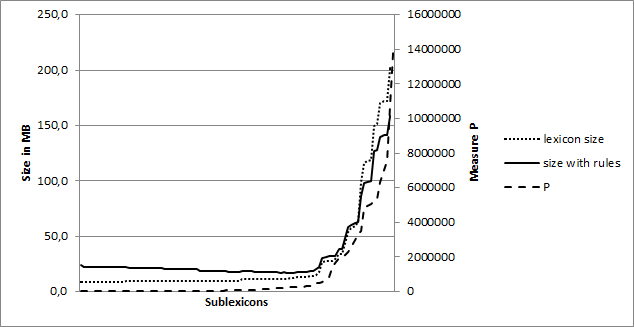
\includegraphics[width=\textwidth]{p-measure.png}
     \caption{Connection between P measure and transducer sizes with flag-diacritics being removed one by one
     \label{fig:p-measure-sizes}}
\end{figure*}

After calculating P for the all sub-lexicons in the Greenlandic lexicon and sorting values, we got data 
that with could be extrapolated by an exponential function. We experimented removing one flag diacritic at a 
time and the sizes we got for the lexicon transducer itself and the one with grammar rules composed is shown in 
figure~\ref{fig:p-measure-sizes}. On the x-axis are sub-lexicons, left y-axis shows sizes in megabytes and the right 
y-axis P-measures. The dotted line shows sizes of the lexicon transducer with flag diacritics removed for 
a sub-lexicon at the time. Each new removal is done to the previous result transducer. Solid dot line shows sizes of the same lexicon transducers with the rules composed to them. 
The dashed line shows P measure (with values on the right y-axis).  
  
It is interesting to see that the relations of P measure and transducer sizes after flag removal somewhat proportional. 
Additionally, the point where the transducer size with the applied rules is the smallest is just after the place where 
the P measure starts rapidly growing. 









In table~\ref{table:sizes} there are shown sizes of the original
transducers compiled with regular lexc compiler composed with grammar rules, transducers compiled
with new method that inserts flag diacritics composed with grammar rules and finally their ratio.

\begin{table}
    \centering
    \begin{tabular}{|l|r|r|r|}
        \hline
        \bf Language & \bf Original & \bf With flags & \bf \% \\
        \hline
        \bf Greenlandic &   168   & 17 & 10,1\%  \\
        \bf North Saami &   12     & 5,7 & 47,5\%  \\
        \bf Finish &   17     & 16 & 94,1\%  \\
        \bf Lule Saami  &   5     & 3 & 60,0\%  \\
        \bf Erzya       &   3,7     & 5,3 & 143,2\%  \\
        \hline
    \end{tabular}
    \caption{Sizes of transducers without and with automatic flags (in megabytes); Percentage shows size of the flagged transducer in comparison to the original
    \label{table:sizes}}
\end{table}


\begin{table}
    \centering
    \begin{tabular}{|l|r|r|r|}
        \hline
        \bf Language & \bf Original & \bf With flags & \bf \% \\
        \hline
        \bf Greenlandic & 2 770 w/s & 2 507 w/s & 90,5\%  \\
        \bf North Saami & 30 714 & 8 775 & 28,6\%  \\
        \bf Finish  & 84 415 & 27 420 & 32,5\%  \\

        \hline
    \end{tabular}
    \caption{Sizes of transducers without and with automatic flags (in megabytes); Percentage shows size of the flagged transducer in comparison to the original
    \label{table:lookup}}
\end{table}


% Find out and discuss why tr with lots of flags get big after applying rules

\section{Data}
\label{sec:data}

We measure the success of our algorithm using real-world, large scale
language descriptions. For this purpose we have acquired freely
available, open source language descriptions from University of
Tromsa's language repository~\cite{moshagen2013building}.\footnote{https://victorio.uit.no/langtech, revision 73836} The
languages selected are Greenlandic (kal), North Saami (sme), Erzya
(myv), Finish (fin) and Lule Sami (smj).

All operations with transducers were performed using Helsinki Finite
State Technology tools~\cite{linden2011}.



\section{Discussion}
\label{sec:discussion}

The results of this study show that large scale language descriptions
can be compiled into smaller transducers using automatically inserted
flags. The effect is especially pronounced for language descriptions
which repeat morphemes in many different places, like the
morphological analyzer for Greenlandic. Since flag diacritics
themselves take space in the transducer graph, this method did not
offer improvements for descriptions where the original
transducer was small.

While requiring {\tt R} flag diacritics will always occur only once
for every left continuation lexicon, the results have shown that, for
certain right continuations, P flag diacritics occur hundreds of
times. This will happen every time when in the same set of morphemes
there are words which have the same beginning. For example, in
figure~\ref{fig:lexc-gr-flag} shows how two morphemes \texttt{maagar}
and \texttt{maagarnar} have same continuation flag
\verb+@P.LEXNAME.IV@+, but they can't collapse into the same path. In future
work, it should be checked if skipping inserting flags for those paths would
further reduce size of transition graphs.


%\subsection{Future Directions}
%\label{subsec:future-directions}

%This is an optimistic thing so we thought that automatic induction of flags
%shoulda work nicely for other neat things too. Hyperminimisation based on
%morphophonology would be cool. Also, graph-structure. And other things.

\section{Conclusion}
\label{sec:conclusion}

In this article we showed that by using morphologically motivated
flags we can dramatically improve the size of the large transducers.  Automatically
inserted flag diacritics would make manual optimization preformed by
linguists unnecessary, which would result in more readable and easier
to maintain linguistic descriptions.

\section{Acknowledgements}
The research leading to these results has received funding from FIN-CLARIN, Langnet and the
European Commission's 7th Framework Program under grant agreement n� 238405 (CLARA).

\bibliographystyle{lrec2014}
\bibliography{lrec2014.bib}




\end{document}
